\documentclass[reqno,12pt]{article}

\usepackage{setspace,graphicx,epstopdf,amsmath,amsfonts,amssymb,amsthm}
\usepackage{datetime,enumitem,subfigure,rotating,fancyvrb}
\usepackage{listings}
\usdate

\begin{document}

\title{\textbf{CS 598 Homework 2}}
  
\author{Mohan Sun\footnote{As usual, the article uses "we" and "our", but the homework is done
by only Mohan "Fred" Sun without any collaboration. Netid: mohans2}}

\date{\vspace{-5ex}}

\maketitle

\doublespacing

\noindent We implement a neural network with a single convolution layer with 5 filters, and train the model
with MNIST data. We achieved an accuracy of 95.13\% which satisfies the requirement. 
Figure \ref{fig:res} shows training results and timing. 

\textit{Model} the model is a modified and extended version of Logisticregression.py. We keep the 
i/o and data processing part, keep the structure of Epoch loop, mini-batch loop, and forward as well as 
backward as function. We modified forward to: 

\begin{lstlisting}
def forward(x,y, model):
    Z = convolution(x, model['K'])
    H = sigmoid(Z)
    U = np.einsum('hijk,ijk',model['W'],H).reshape( \
        model['W'].shape[0],1) + model['b']
    p = softmax_function(U)
    return Z, H, p
\end{lstlisting}

\newpage
and backward to:

\begin{lstlisting}
def backward(x, y, Z, H, p, model, model_grads):
    dU = np.copy(p)
    dU[y] = dU[y] - 1
    delta = np.einsum('hijk,h',model['W'], \
        dU.reshape(dU.shape[0]))
    dK = convolution(x, delta * sigmoidp(Z))
    dW = np.zeros_like(model['W'])
    for i in range(dW.shape[0]):
        dW[i,:,:,:] = dU[i] * H
    model_grads['W']=dW
    model_grads['b']=dU
    model_grads['K']=dK
    return model_grads
\end{lstlisting}

\newpage
we also add a convolution function:
\begin{lstlisting}
def convolution(X, K):
    dx, dy = X.shape
    kx, ky, p = K.shape
    ans = np.zeros((dx-kx+1,dy-ky+1,p))
    for k in range(ans.shape[2]):
        for j in range(ans.shape[1]):
            for i in range(ans.shape[0]):
                ans[i,j,k] = np.einsum('ij,ij', \
                    X[i:i+kx,j:j+ky], K[:,:,k])
    return ans
\end{lstlisting}

We still use sigmoid as ReLU tend to go overflow in softmax function.

\textit{parameters} For this model, we define $\mathbf{K} \in \mathbb{R}^{k_x \times k_y \times C},\, k_x=k_y=5, C = 5$ 
and $LR^{(0)}=0.1$. $LR$ is scaled down by $10$ for every $5$ epochs.

\begin{figure}[!t]
  \centering 
  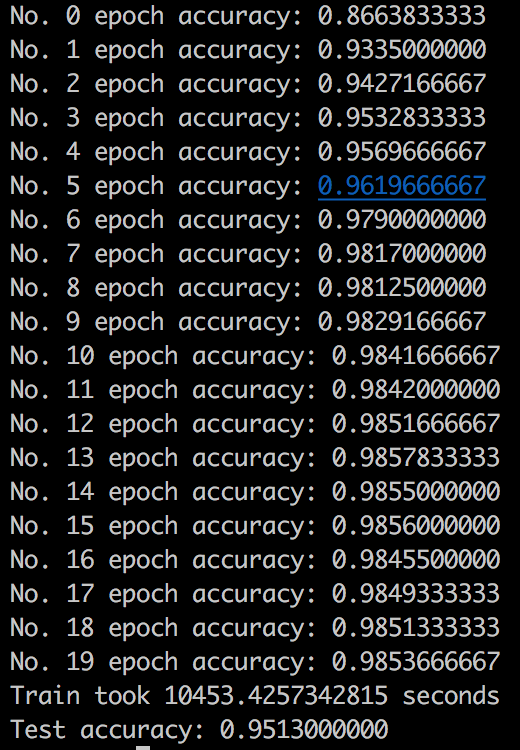
\includegraphics[width = \textwidth]{HW2_result.png}

  \vskip0.25cm

  \caption{\textnormal{\bf Neural Network Training Result and Timing.} 
  Training takes approximately 10453 seconds. We achieved an accuracy of 95.13\%}
  \label{fig:res}
\end{figure}

\end{document}
